\chapter{Pengenalan OpenCV}
\section{OpenCV}
\subsection{Definisi OpenCV}
	
	Computer Vision adalah ilmu pemrograman komputer untuk memproses dan pada akhirnya memahami gambar dan video, atau hanya mengatakan membuat komputer melihatnya. Memecahkan sebagian kecil dari tantangan Visi Komputer tertentu, menciptakan kemungkinan baru yang menarik dalam teknologi, teknik, dan bahkan hiburan. Untuk memajukan penelitian visi dan menyebarkan pengetahuan visi, sangat penting untuk memiliki perpustakaan fungsi pemrograman dengan kode yang dioptimalkan dan portabel, dan mudah-mudahan tersedia secara gratis. Ini adalah tujuan asli tim Intel pada tahun 1999 ketika OpenCV (Open Source Computer Vision Library) secara resmi diluncurkan. Sejak itu, sejumlah programmer telah berkontribusi pada perkembangan perpustakaan terbaru. Perubahan besar terbaru terjadi pada tahun 2009 (OpenCV 2) yang mencakup perubahan utama pada antarmuka C ++. Rilis perpustakaan terbaru dapat ditemukan di situs web resmi OpenCV. Saat ini perpustakaan memiliki> 2500 algoritma yang dioptimalkan. Ini digunakan secara luas di seluruh dunia, memiliki> 2,5 juta unduhan dan> 40 ribu orang di grup pengguna. OpenCV dapat digunakan dalam aplikasi akademik dan komersial juga, di bawah lisensi BSD. Untuk menguasai setiap elemen pustaka OpenCV perlu berkonsultasi dengan banyak buku yang tersedia tentang topik OpenCV. Namun demikian, membaca materi yang lebih komprehensif seperti itu harus lebih mudah setelah memahami ide dasar tentang OpenCV dari makalah ini. Bahkan untuk membuatnya lebih nyaman, teks yang disajikan di sini dengan cermat mengikuti salah satu sumber OpenCV terbaru.

	OpenCV adalah pustaka Pengolah Gambar yang dibuat oleh Intel, dapat diunduh secara bebas dan tersedia untuk C, C ++, Java dan Python, Windows, Linux, Mac OS, iOS dan Android Terbaru Versi-versinya adalah opencv2.4.13 dan opencv-3.1. Ini adalah Sumber terbuka dan juga Mudah digunakan dan diinstal. Ini dirancang untuk efisiensi komputasi fokus yang kuat pada aplikasi waktu nyata Implementasi pertama adalah dalam bahasa pemrograman C; Namun, popularitasnya tumbuh dengan implementasi C ++ pada Versi 2.0. Fungsi baru diprogram dengan C ++. Namun, saat ini, perpustakaan memiliki antarmuka penuh untuk bahasa pemrograman lain, seperti Java, Python, dan MATLAB / Octave. OpenCV tersedia secara bebas untuk diunduh di http://opencv.org. Situs ini menyediakan versi terakhir untuk distribusi (saat ini, 3.0 beta) dan versi yang lebih lama. OpenCV mengharuskan gambar dalam BGR atau Grayscale untuk ditampilkan atau disimpan. Kalau tidak, efek yang tidak diinginkan dapat terjadi.

	Pustaka OpenCV (sejak versi 2.2) dibagi menjadi beberapa modul, di mana setiap modul dapat dipahami, secara umum, sebagai didedikasikan untuk satu kelompok masalah penglihatan komputer. Semua kelas dan fungsi didefinisikan dalam ruang nama cv. Oleh karena itu untuk mengaksesnya kita dapat mendahului definisi fungsi utama dengan deklarasi menggunakan namespace cv; atau awali nama kelas dan fungsi OpenCV berdasarkan spesifikasi namespace cv. Objek utama adalah Mat kelas. Seperti dilibatkan oleh nama kelas itu pada dasarnya adalah sebuah matriks yang memegang nilai-nilai piksel dari beberapa gambar dan, di samping itu, sejumlah atribut tentang suatu gambar. Dalam kasus yang paling sederhana, sebuah gambar dapat dibuat sebagai cv :: Mat image ;, membuat gambar dengan ukuran 0 x 0. Mungkin variabel anggota yang paling penting dari objek gambar adalah data di mana anggota image.data sebenarnya adalah penunjuk ke memori yang dialokasikan blok yang berisi data gambar (dalam kasus sepele ini adalah image.data = 0). Atau selama pembuatan objek Mat kita bisa secara eksplisit menentukan ukuran awal dan jenis setiap elemen matriks. Jenis ini menentukan, misalnya, menandatangani nilai gambar piksel 1-byte, atau tiga saluran untuk gambar berwarna , atau bahkan angka titik apung 32-bit atau 64bit.

	Setelah objek matematika kelas didefinisikan, fitur yang bagus tentangnya (tidak ada dalam versi awal OpenCV) adalah bahwa alokasi / deallokasi memori dilakukan secara otomatis. Misalnya, memori yang secara otomatis dialokasikan selama gambar dibacakan ke beberapa objek, juga akan secara otomatis dirilis setelah objek yang sesuai keluar dari ruang lingkup. Hal penting lainnya adalah bahwa kelas Mat mengimplementasikan penghitungan referensi dan salinan dangkal. Oleh karena itu, ketika gambar ditugaskan ke yang lain, data gambar itu sendiri tidak disalin dan kedua gambar menunjuk ke blok memori yang sama (ini juga berlaku untuk gambar yang dilewati / dikembalikan oleh nilai). Namun, karena jumlah referensi didukung, memori yang dialokasikan untuk data gambar (piksel) itu sendiri akan dirilis hanya ketika semua referensi ke gambar dihancurkan.

	Dalam versi sebelum OpenCV 2, fungsi dan struktur seperti C digunakan (masih bisa jadi) dan struktur utama adalah IplImage. Meskipun ada cara mudah untuk mengubah struktur IplImage menjadi objek cv :: Mat, sangat disarankan untuk menghindari struktur data yang sudah usang ini.

\newpage
\subsection{Sejarah Kecerdasan Opencv}
    Resmi diluncurkan pada tahun 1999, proyek OpenCV pada awalnya merupakan inisiatif Intel Research untuk memajukan aplikasi intensif CPU, bagian dari serangkaian proyek termasuk penelusuran sinar waktu nyata dan dinding layar 3D. Kontributor utama untuk proyek ini termasuk sejumlah pakar optimisasi di Intel Rusia, serta Tim Perpustakaan Kinerja Intel. Pada hari-hari awal OpenCV, tujuan proyek digambarkan sebagai:

    \begin{enumerate}
	\item Memajukan penelitian visi dengan menyediakan tidak hanya kode terbuka tetapi juga dioptimalkan untuk infrastruktur visi dasar. Tidak ada lagi menciptakan kembali roda.
	\item Menyebarkan pengetahuan visi dengan menyediakan infrastruktur umum yang dapat dibangun oleh pengembang, sehingga kode akan lebih mudah dibaca dan dapat ditransfer.
	\item Aplikasi komersial berbasis visi mutakhir dengan membuat kode portabel yang dioptimalkan kinerja tersedia secara gratis - dengan lisensi yang tidak memerlukan kode untuk terbuka atau bebas sendiri.
	\end{enumerate} 

	Versi alpha pertama dari OpenCV dirilis ke publik di Konferensi IEEE pada Computer Vision dan Pattern Recognition pada tahun 2000, dan lima beta dirilis antara tahun 2001 dan 2005. Versi 1.0 pertama dirilis pada tahun 2006. Versi 1.1 "pra-rilis "dirilis pada Oktober 2008.

	Rilis utama kedua dari OpenCV adalah pada Oktober 2009. OpenCV 2 mencakup perubahan besar pada antarmuka C ++, yang bertujuan untuk lebih mudah, pola yang lebih aman, fungsi baru, dan implementasi yang lebih baik untuk yang sudah ada dalam hal kinerja (terutama pada multi- sistem inti). Rilis resmi sekarang terjadi setiap enam bulan dan pengembangan sekarang dilakukan oleh tim Rusia independen yang didukung oleh perusahaan komersial.

	Pada Agustus 2012, dukungan untuk OpenCV diambil alih oleh yayasan nirlaba OpenCV.org, yang mengelola pengembang dan situs pengguna.

	Pada Mei 2016, Intel menandatangani perjanjian untuk mengakuisisi Itseez, pengembang OpenCV terkemuka.

\newpage
\section{NumPy}
\subsection{Definisi NumPy}
NumPy adalah perpustakaan untuk bahasa pemrograman Python, menambahkan dukungan untuk array dan matriks multi-dimensi yang besar, bersama dengan koleksi besar fungsi matematika tingkat tinggi untuk beroperasi pada array ini. Nenek moyang NumPy, Numeric, pada awalnya diciptakan oleh Jim Hugunin dengan kontribusi dari beberapa pengembang lainnya. Pada 2005, Travis Oliphant menciptakan NumPy dengan memasukkan fitur-fitur Numarray yang bersaing ke Numeric, dengan modifikasi ekstensif. NumPy adalah perangkat lunak sumber terbuka dan memiliki banyak kontributor.

\subsection{Sejarah NumPy}
Bahasa pemrograman Python pada awalnya tidak dirancang untuk komputasi numerik, tetapi menarik perhatian komunitas ilmiah dan teknik sejak awal, sehingga kelompok minat khusus yang disebut matrix-sig didirikan pada tahun 1995 dengan tujuan mendefinisikan paket komputasi array. Di antara anggotanya adalah desainer dan pengelola Python, Guido van Rossum, yang menerapkan ekstensi ke sintaksis Python (khususnya sintaks pengindeksan) untuk membuat komputasi array lebih mudah.

Implementasi dari paket matriks diselesaikan oleh Jim Fulton, kemudian digeneralisasi oleh Jim Hugunin menjadi Numeric, juga beragam disebut ekstensi Numerical Python atau NumPy. Hugunin, seorang mahasiswa pascasarjana di Massachusetts Institute of Technology (MIT), bergabung dengan Corporation for National Research Initiatives (CNRI) untuk bekerja pada JPython pada tahun 1997 meninggalkan Paul Dubois dari Lawrence Livermore National Laboratory (LLNL) ke ambil alih sebagai pengelola. Kontributor awal lainnya termasuk David Ascher, Konrad Hinsen dan Travis Oliphant.

Paket baru bernama Numarray ditulis sebagai pengganti Numeric yang lebih fleksibel. Seperti Numeric, sekarang sudah usang. Numarray memiliki operasi lebih cepat untuk array besar, tetapi lebih lambat daripada Numeric pada array kecil, jadi untuk sementara waktu kedua paket digunakan untuk kasus penggunaan yang berbeda. Versi terakhir Numeric v24.2 dirilis pada 11 November 2005 dan numarray v1.5.2 dirilis pada 24 Agustus 2006.

Ada keinginan untuk memasukkan Numeric ke dalam pustaka standar Python, tetapi Guido van Rossum memutuskan bahwa kodenya tidak dapat dipertahankan dalam keadaannya saat itu.

Pada awal 2005, pengembang NumPy Travis Oliphant ingin menyatukan komunitas sekitar satu paket array dan mem-porting fitur Numarray ke Numeric, merilis hasilnya sebagai NumPy 1.0 pada 2006. Proyek baru ini adalah bagian dari SciPy. Untuk menghindari menginstal paket SciPy besar hanya untuk mendapatkan objek array, paket baru ini dipisahkan dan disebut NumPy. Dukungan untuk Python 3 ditambahkan pada 2011 dengan NumPy versi 1.5.0.

Pada tahun 2011, PyPy memulai pengembangan penerapan API NumPy untuk PyPy. Ini belum sepenuhnya kompatibel dengan NumPy.

\subsection{Perkembangan NumPy}
NumPy menargetkan implementasi referensi CPython dari Python, yang merupakan penerjemah bytecode yang tidak mengoptimalkan. Algoritma matematika yang ditulis untuk versi Python ini sering berjalan jauh lebih lambat daripada yang dikompilasi setara. NumPy mengatasi masalah kelambatan sebagian dengan menyediakan array multidimensi dan fungsi dan operator yang beroperasi secara efisien pada array, membutuhkan penulisan ulang beberapa kode, sebagian besar loop internal menggunakan NumPy.

Menggunakan NumPy dalam Python memberikan fungsionalitas yang sebanding dengan MATLAB karena keduanya diinterpretasikan, dan keduanya memungkinkan pengguna untuk menulis program cepat selama sebagian besar operasi bekerja pada array atau matriks, bukan skalar. Sebagai perbandingan, MATLAB menawarkan sejumlah besar kotak alat tambahan, terutama Simulink, sedangkan NumPy secara intrinsik terintegrasi dengan Python, bahasa pemrograman yang lebih modern dan lengkap. Selain itu, paket Python komplementer tersedia; SciPy adalah pustaka yang menambahkan lebih banyak fungsi seperti MATLAB dan Matplotlib adalah paket merencanakan yang menyediakan fungsi merencanakan seperti MATLAB. Secara internal, baik MATLAB dan NumPy mengandalkan BLAS dan LAPACK untuk perhitungan aljabar linier yang efisien.

Binding Python dari perpustakaan visi komputer yang banyak digunakan OpenCV memanfaatkan array NumPy untuk menyimpan dan beroperasi pada data. Karena gambar dengan banyak saluran hanya direpresentasikan sebagai array tiga dimensi, pengindeksan, pemotongan atau penutupan dengan array lainnya adalah cara yang sangat efisien untuk mengakses piksel tertentu dari suatu gambar. Array NumPy sebagai struktur data universal dalam OpenCV untuk gambar, poin fitur yang diekstraksi, filter kernel dan banyak lagi yang sangat menyederhanakan alur kerja pemrograman dan debugging.

\textbf{Struktur data ndarray}
\newline
Fungsionalitas inti dari NumPy adalah ndarray, untuk susunan n-dimensional, struktur data. Array-array ini adalah pandangan yang melintas pada memori. Berbeda dengan struktur data daftar built-in Python (yang, meskipun namanya, adalah array dinamis), array ini diketik secara homogen: semua elemen dari array tunggal harus dari tipe yang sama.

Array tersebut juga dapat dilihat ke buffer memori yang dialokasikan oleh ekstensi C atau C plus plus, Cython, dan Fortran ke juru bahasa CPython tanpa perlu menyalin data, memberikan tingkat kompatibilitas dengan perpustakaan numerik yang ada. Fungsi ini dieksploitasi oleh paket SciPy, yang membungkus sejumlah perpustakaan seperti itu (terutama BLAS dan LAPACK). NumPy memiliki dukungan bawaan untuk ndarrays yang dipetakan di memori.

\textbf{Keterbatasan}
\newline
Memasukkan atau menambahkan entri ke sebuah array tidak sepele mungkin dengan daftar Python. Rutin np.pad untuk memperluas array sebenarnya membuat array baru dengan nilai bentuk dan padding yang diinginkan, menyalin array yang diberikan ke yang baru dan mengembalikannya. Operasi NumPy np.concatenate tidak benar-benar menghubungkan dua array tetapi mengembalikan yang baru, diisi dengan entri dari kedua array yang diberikan secara berurutan. Membentuk kembali dimensi array dengan np.reshape hanya mungkin selama jumlah elemen dalam array tidak berubah. Keadaan ini berasal dari fakta bahwa array NumPy harus dilihat pada buffer memori yang berdekatan. Paket pengganti yang disebut Blaze berupaya mengatasi batasan ini. 

Algoritma yang tidak dapat diekspresikan sebagai operasi vektor biasanya akan berjalan lambat karena mereka harus diimplementasikan dalam Python murni, sedangkan vektorisasi dapat meningkatkan kompleksitas memori dari beberapa operasi dari konstan ke linier, karena array sementara harus dibuat yang sama besarnya dengan input. Kompilasi kode numerik Runtime telah diterapkan oleh beberapa kelompok untuk menghindari masalah ini; solusi open source yang beroperasi dengan NumPy termasuk scipy.weave, numexpr dan Numba. Cython dan Pythran adalah alternatif kompilasi statis untuk ini.

\newpage
\subsection{Contoh Code Numpy}
Membuat Array menggunakan Numpy Python
\lstinputlisting{src/MembuatArray.py}

Operasi Sederhana Numpay
\lstinputlisting{src/OperasiSederhana.py}

Fungsi Universal Numpay
\lstinputlisting{src/UniversalFunction.py}

Aljabar Linear bagaimana memuat matriks menggunakan code numpay dengan mudah.
\lstinputlisting{src/LinearAlgebra.py}

Contoh penggabungan Numpay dengan Opencv.
\lstinputlisting{src/Penggabungan.py}	

\newpage
\section{Instalasi OpenCV}
\subsection{Instalasi pada Windows}

Windows tidak datang dengan Python yang sudah diinstal. Namun, wizard instalasi tersedia untuk Python, NumPy, SciPy, dan OpenCV yang telah dikompilasi. Atau, kita dapat membangun dari sumber. Sistem build OpenCV menggunakan CMake untuk konfigurasi dan Visual Studio atau MinGW untuk kompilasi.

Jika kami ingin dukungan untuk kamera kedalaman, termasuk Kinect, pertama-tama kita harus menginstal OpenNI dan SensorKinect, yang tersedia sebagai binari yang dikompilasi dengan wizard penginstalan. Kemudian, kita harus membangun OpenCV dari sumber.

\textbf{Catatan}

Versi OpenCV yang dikompilasi sebelumnya tidak menawarkan dukungan untuk kamera yang dalam. Pada Windows, OpenCV 2 menawarkan dukungan yang lebih baik untuk Python 32-bit daripada Python 64-bit. namun, dengan mayoritas komputer yang dijual hari ini menggunakan sistem 64-bit, instruksi kami akan merujuk pada 64-bit. Semua installer memiliki versi 32-bit yang tersedia dari situs yang sama dengan 64-bit.

\begin{enumerate}
	\item Beberapa langkah berikut merujuk pada pengeditan variabel PATH sistem. Tugas ini dapat dilakukan di jendela Variabel Lingkungan di Panel Kontrol.
	\item Pada Windows Vista / Windows 7 / Windows 8, klik menu Start dan luncurkan Panel Kontrol. Sekarang, navigasikan ke System and Security, Sistem, Pengaturan sistem lanjutan. Klik pada tombol Variabel Lingkungan….
	\item Pada Windows XP, klik pada menu Mulai dan navigasikan ke Control Panel | Sistem. Pilih tab Advanced. Klik pada tombol Variabel Lingkungan….
	\item Sekarang, di bawah System variable, pilih Path dan klik tombol Edit….
	\item Buat perubahan sesuai petunjuk.
	\item Untuk menerapkan perubahan, klik pada semua tombol OK (sampai kita kembali ke jendela utama Control Panel).
	\item Kemudian, keluar dan masuk kembali (atau reboot).
\end{enumerate}

\newpage
\textbf{Menggunakan penginstal biner (tidak ada dukungan untuk kamera kedalaman)}

Anda dapat memilih untuk menginstal Python dan pustaka terkait secara terpisah jika Anda mau; Namun, ada distribusi Python yang datang dengan installer yang akan mengatur seluruh tumpukan SciPy (yang mencakup Python dan NumPy), yang membuatnya sangat sepele untuk mengatur lingkungan pengembangan.
	
Salah satu distribusi tersebut adalah Anaconda Python (dapat diunduh di ). Setelah installer diunduh, jalankan dan ingat untuk menambahkan path ke instalasi Anaconda ke variabel PATH Anda mengikuti prosedur sebelumnya.

Berikut adalah langkah-langkah untuk mengatur Python7, NumPy, SciPy, dan OpenCV:
\begin{enumerate}
	\item Unduh dan instal 64 bit Python 3.7.1 dari \begin{verbatim} https://www.python.org/ftp/python/3.7.1/python-3.7.1-amd64.exe \end{verbatim}
		\begin{figure}[ht]
		\centering
		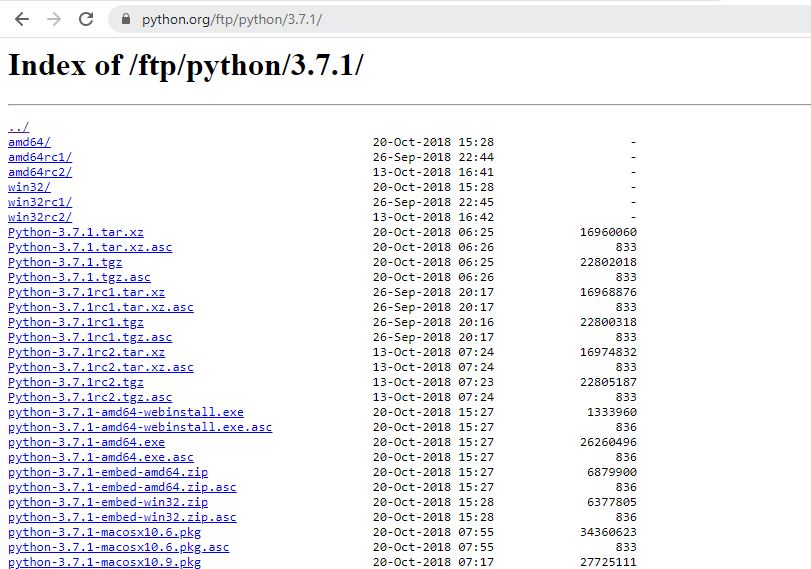
\includegraphics[scale=0.5]{figures/1,1.jpg}
		\caption{Download Python}
		\label{contoh}
		\end{figure}
\newpage
	\item Unduh dan instal NumPy 1.6.2.
		\begin{figure}[ht]
		\centering
		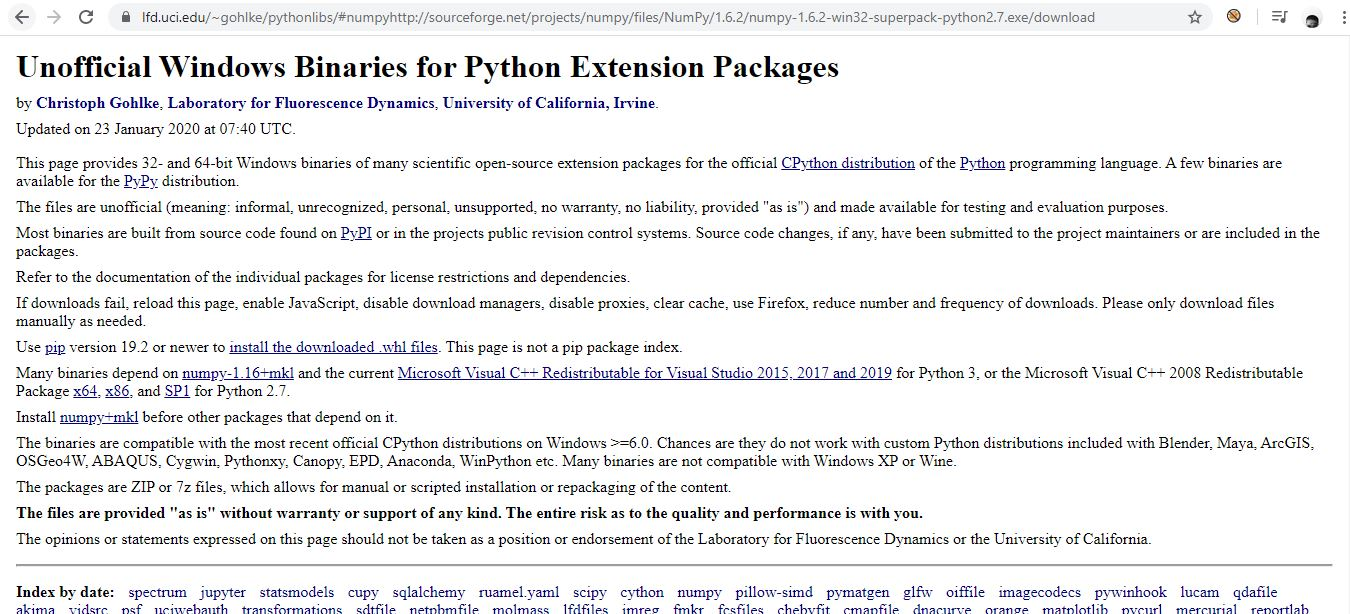
\includegraphics[scale=0.5]{figures/1,2.jpg}
		\caption{Cari Numpy terbaru pada wibsite ini}
		\label{contoh}
		\end{figure}
\newpage
	\item Unduh dan pasang SciPy 11.0 dari \begin{verbatim} http://www.lfd.uci.edu/~gohlke/pythonlibs/#scipyhttp://sourceforge.net/projects/scipy/files/scipy/0.11.0/scipy0.11.0win32-superpack-python2.7.exe/download \end{verbatim} (ini sama dengan NumPy dan ini adalah pemasang komunitas).
		\begin{figure}[ht]
		\centering
		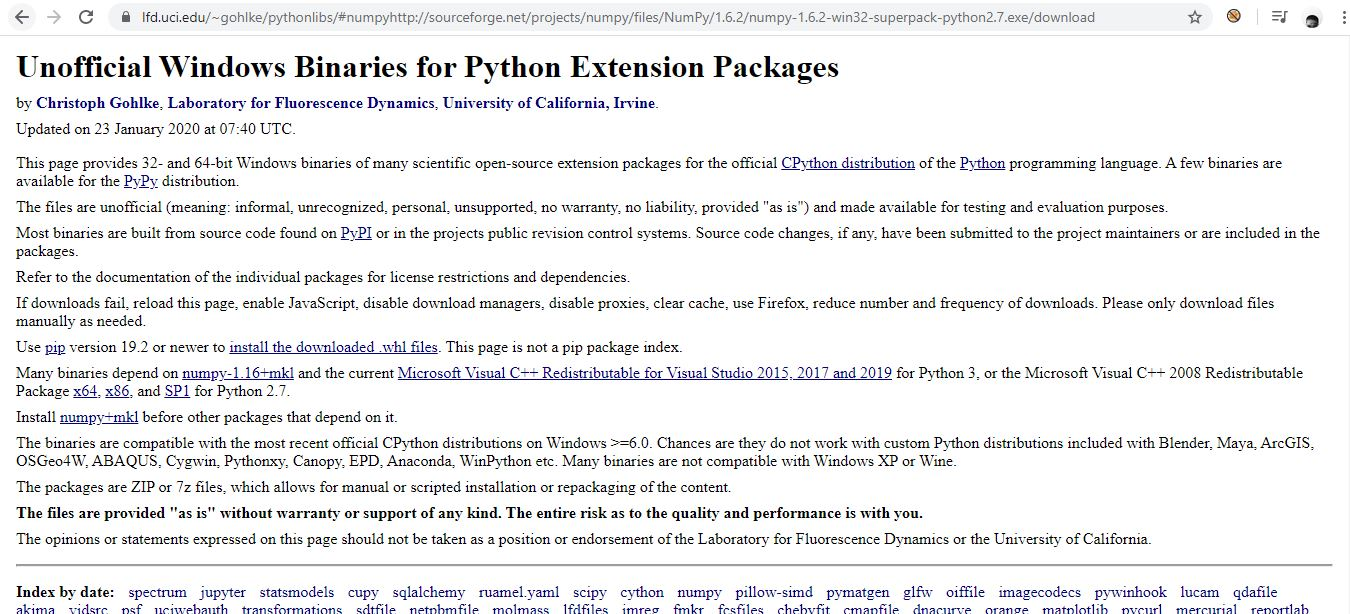
\includegraphics[scale=0.5]{figures/1,2.jpg}
		\caption{Cari SciPy Terbaru pada website ini}
		\label{contoh}
		\end{figure}
	\item Unduh ZIP self-extracting dari OpenCV 3.0.0 dari \begin{verbatim} https://github.com/Itseez/opencv \end{verbatim}. Jalankan ZIP ini, dan ketika diminta, masukkan folder tujuan. 
	\item Salin \begin{verbatim} <unzip_destination>\opencv\build\python\2.7\cv2.pyd \end{verbatim} ke \begin{verbatim} C:\Python2.7\Lib\site-packages \end{verbatim} (dengan asumsi bahwa kami telah menginstal Python 2.7 ke lokasi default). Jika Anda menginstal Python 2.7 dengan Anaconda, gunakan folder instalasi Anaconda daripada instalasi Python default. Sekarang, instalasi Python baru dapat menemukan OpenCV.
	\item Langkah terakhir diperlukan jika kita ingin skrip Python dijalankan menggunakan instalasi Python baru secara default. Edit variabel PATH sistem dan tambahkan C: /Python2.7 (dengan asumsi kami telah menginstal Python 2.7 ke lokasi default) atau folder instalasi Anaconda Anda. Hapus jalur Python sebelumnya, seperti C:/Python2.6. Logout dan login kembali (sebagai alternatif, reboot).
\end{enumerate}

\newpage
\textbf{Menggunakan CMake dan kompiler}

Windows tidak dilengkapi dengan kompiler atau CMake. Kita perlu menginstalnya. Jika kami ingin dukungan untuk kamera kedalaman, termasuk Kinect, kami juga perlu menginstal OpenNI dan SensorKinect.

Mari kita asumsikan bahwa kita telah menginstal Python 2.7, NumPy, dan SciPy 32-bit baik dari binari (seperti dijelaskan sebelumnya) atau dari sumber. Sekarang, kita dapat melanjutkan dengan menginstal kompiler dan CMake, menginstal opsional OpenNI dan SensorKinect, dan kemudian membangun OpenCV dari sumber:

\begin{enumerate}
	\item Unduh dan instal CMake 3.1.2 dari \begin{verbatim} http://www.cmake.org/files/v3.1/cmake3.1.2-win32-x86.exe \end{verbatim} 
		\begin{figure}[ht]
		\centering
		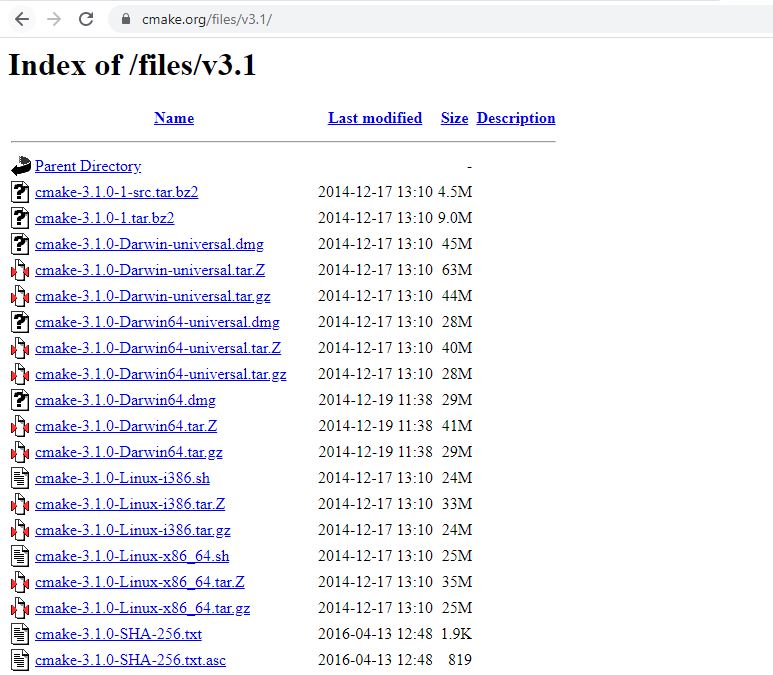
\includegraphics[scale=0.5]{figures/1,3.jpg}
		\caption{Cari CMake Terbaru pada website ini kemudian install}
		\label{contoh}
		\end{figure}
	Saat menjalankan penginstal, pilih Tambahkan CMake ke PATH sistem untuk semua pengguna atau Tambahkan CMake ke PATH sistem untuk pengguna saat ini. Jangan khawatir tentang fakta bahwa CMake versi 64-bit tidak tersedia, CMake hanyalah alat konfigurasi dan tidak melakukan kompilasi apa pun. Sebaliknya, pada Windows, itu menciptakan file proyek yang dapat dibuka dengan Visual Studio.
\newpage
	\item Unduh dan instal Microsoft Visual Studio 2013 (edisi Desktop jika Anda bekerja pada Windows 7) dari \begin{verbatim}https://www.visualstudio.com/products/free-developeroffers-vs.aspx?slcid=0x409&type=web or MinGW \end{verbatim} 
		\begin{figure}[ht]
		\centering
		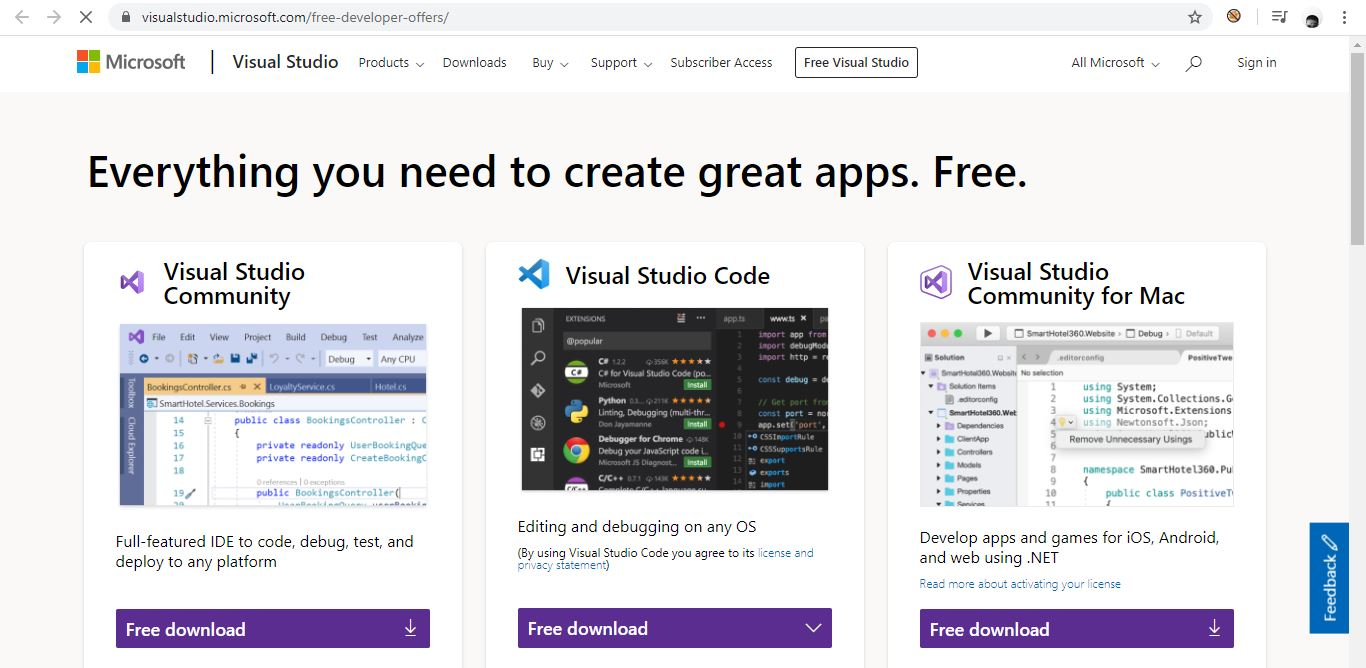
\includegraphics[scale=0.3]{figures/1,4.jpg}
		\caption{Cari VisualStudio Terbaru pada website ini kemudian install}
		\label{contoh}
		\end{figure}
	Perhatikan bahwa Anda harus masuk dengan akun Microsoft Anda dan jika Anda tidak memilikinya, Anda dapat membuatnya di tempat. Instal perangkat lunak dan reboot setelah instalasi selesai. 
\newpage
	\textbf{Untuk MinGW, dapatkan penginstalnya dari} \begin{verbatim}http://sourceforge.net/projects/mingw/files/Installer/mingw-get-setup.exe/download \end{verbatim} 
		\begin{figure}[ht]
		\centering
		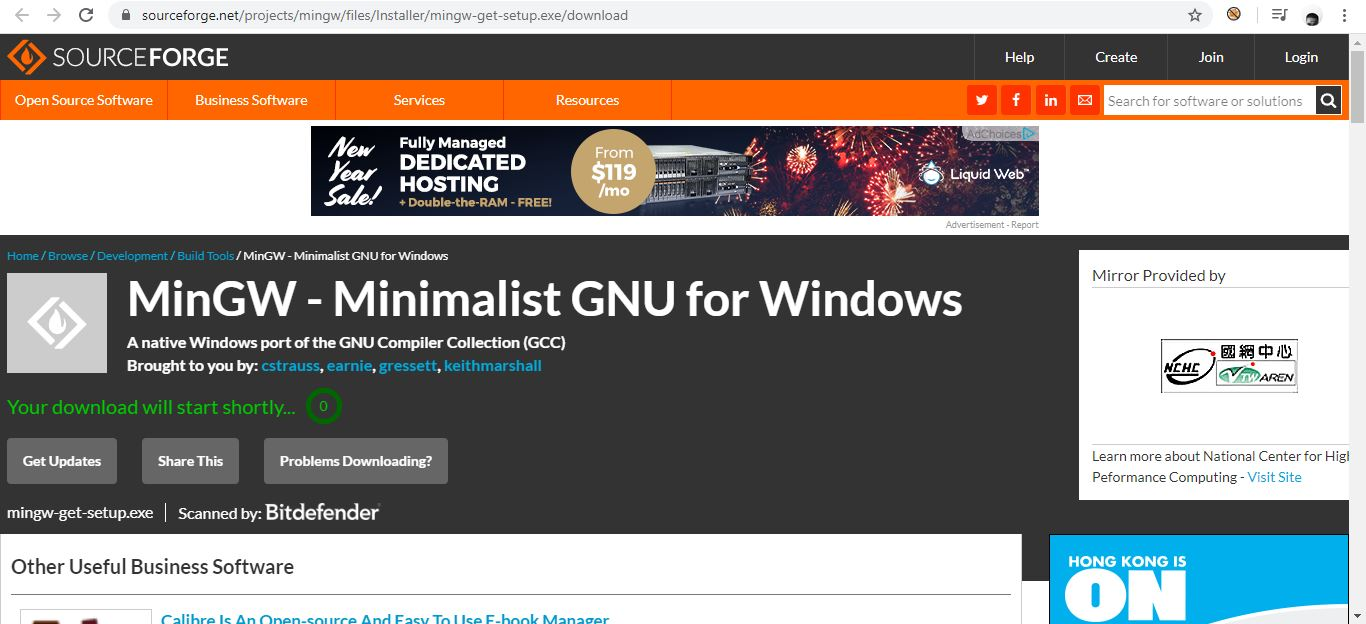
\includegraphics[scale=0.3]{figures/1,5.jpg}
		\caption{Download MinGW}
		\label{contoh}
		\end{figure}
	dan \begin{verbatim}http://sourceforge.net/projects/mingw/files/OldFiles/mingw-get-inst/mingw-getinst-20120426/mingw-get-inst-20120426.exe/download \end{verbatim} 
\newpage
		\begin{figure}[ht]
		\centering
		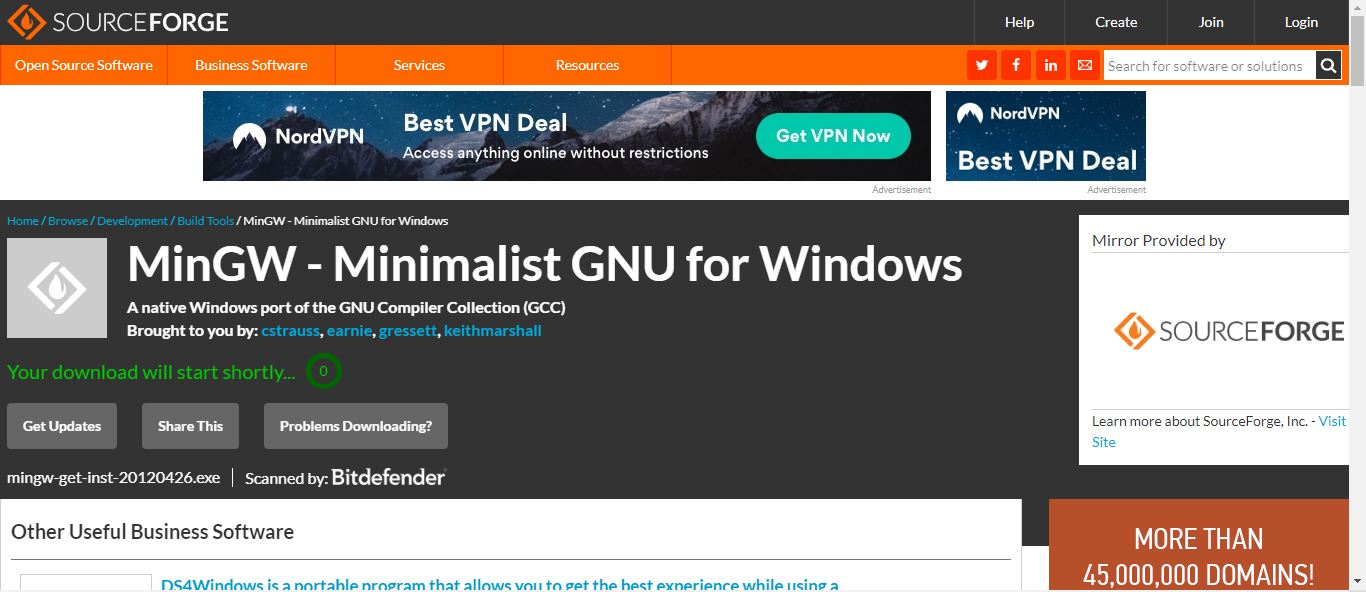
\includegraphics[scale=0.3]{figures/1,6.jpg}
		\caption{Download MinGW}
		\label{contoh}
		\end{figure}
	Saat menjalankan penginstal, pastikan jalur tujuan tidak mengandung spasi dan bahwa kompiler C ++ opsional disertakan. Edit variabel PATH sistem dan tambahkan; \begin{verbatim}C:\MinGW\bin \end{verbatim} (dengan asumsi MinGW diinstal ke lokasi default). Mulai ulang sistem.
	\item Secara opsional, unduh dan instal OpenNI 1.5.4.0 dari tautan yang disediakan di beranda GitHub di OpenNI di \begin{verbatim}https://github.com/OpenNI/OpenNI \end{verbatim}
\newpage
		\begin{figure}[ht]
		\centering
		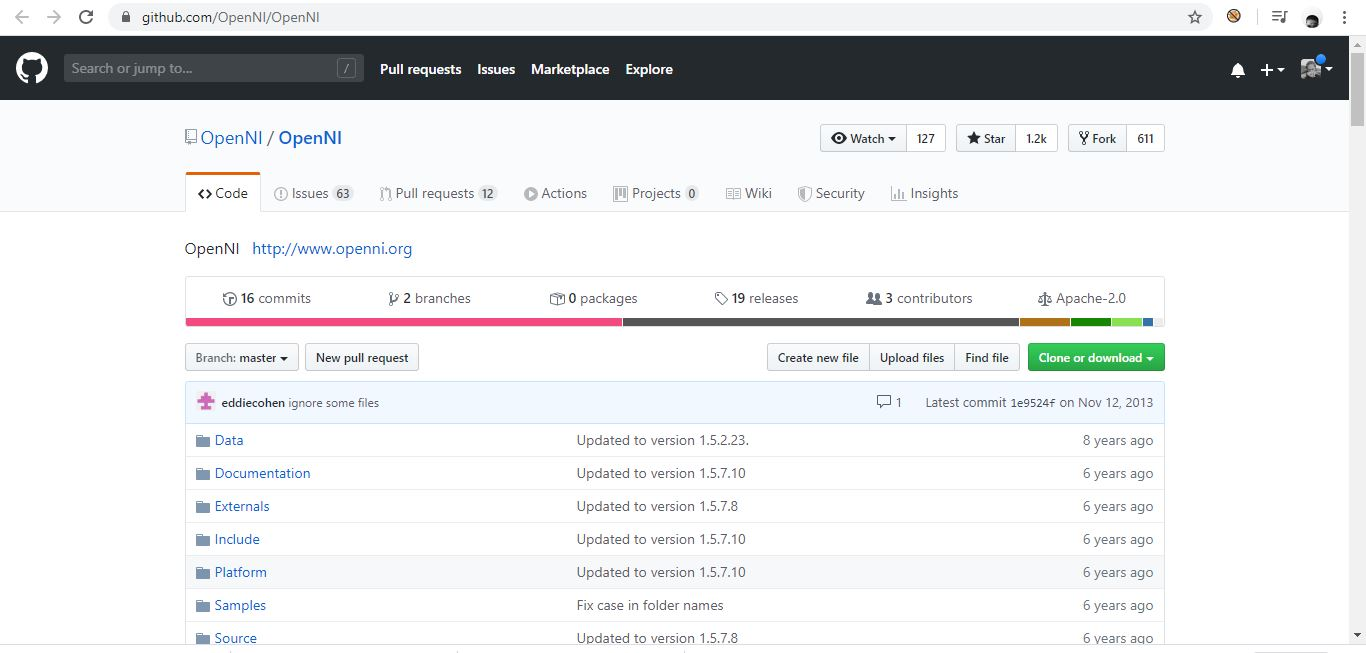
\includegraphics[scale=0.3]{figures/1,7.jpg}
		\caption{Download OpenNI}
		\label{contoh}
		\end{figure}
	\item Anda dapat mengunduh dan menginstal SensorKinect 0.93 dari \begin{verbatim}https://github.com/avin2/SensorKinect/blob/unstable/Bin/SensorKinect093-BinWin32-v5.1.2.1.msi?raw=true (32-bit) \end{verbatim} 
		\begin{figure}[ht]
		\centering
		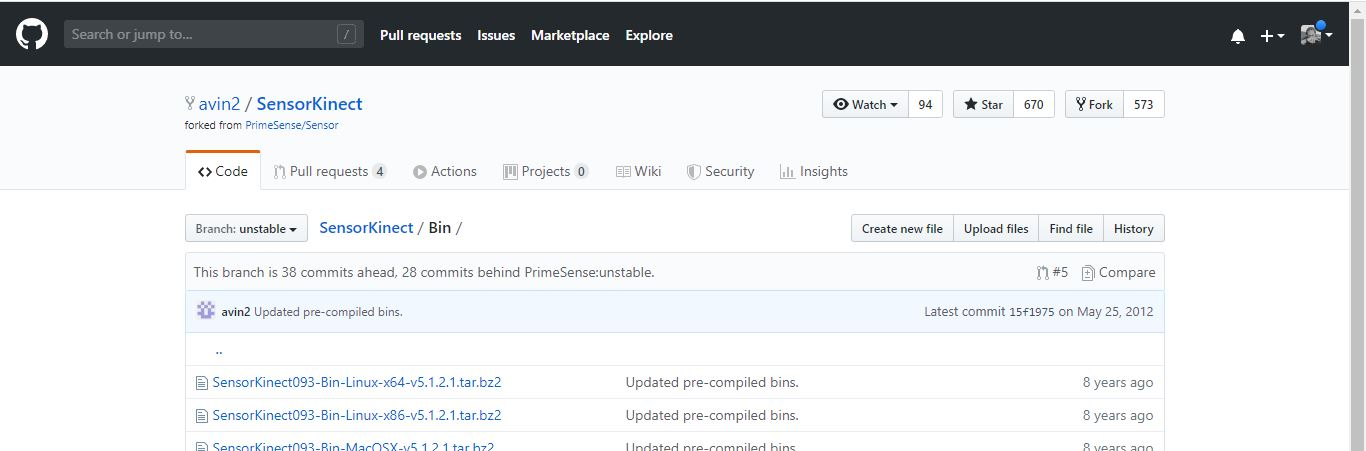
\includegraphics[scale=0.3]{figures/1,8.jpg}
		\caption{Download SensorKinect}
		\label{contoh}
		\end{figure}
\newpage
	Atau, untuk Python 64-bit, unduh di \begin{verbatim} https://github.com/avin2/SensorKinect/blob/unstable/Bin/SensorKinect093-BinWin64-v5.1.2.1.msi?raw=true \end{verbatim}(64-bit). 
		\begin{figure}[ht]
		\centering
		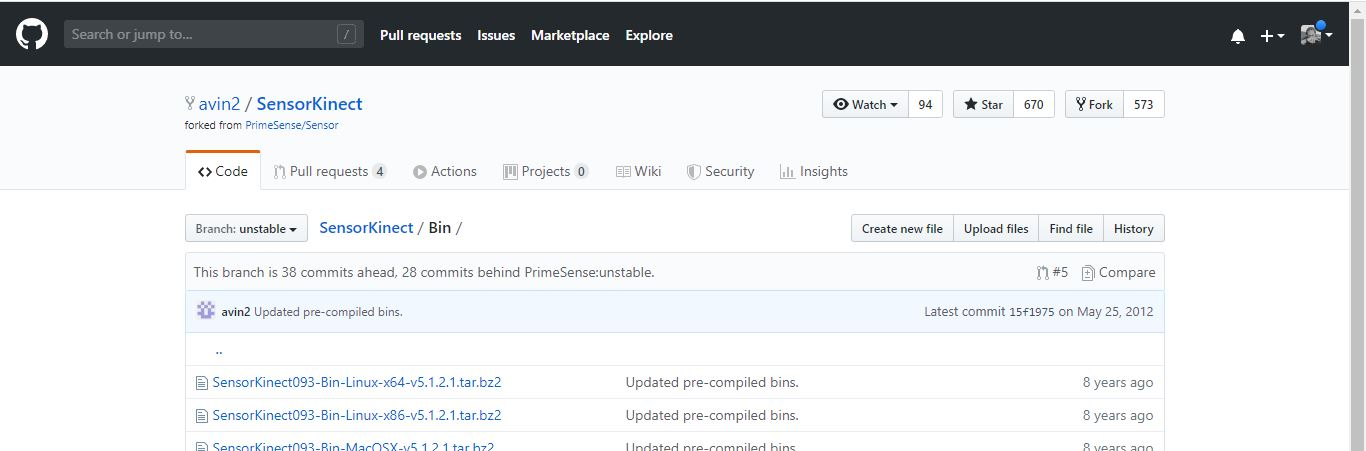
\includegraphics[scale=0.3]{figures/1,8.jpg}
		\caption{Download SensorKinect}
		\label{contoh}
		\end{figure}
	Perhatikan bahwa repositori ini tidak aktif selama lebih dari tiga tahun.
	\item Unduh ZIP self-extracting dari OpenCV 3.0.0 dari \begin{verbatim}https://github.com/Itseez/opencv \end{verbatim} 
		\begin{figure}[ht]
		\centering
		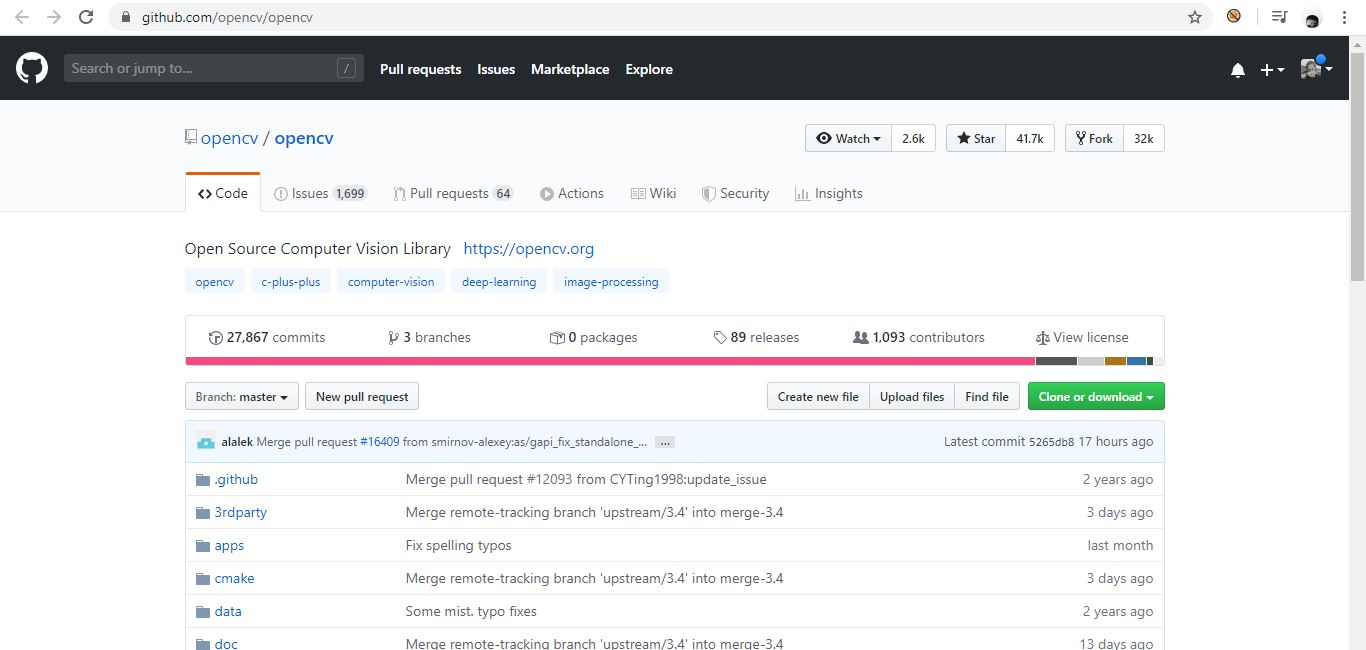
\includegraphics[scale=0.3]{figures/1,9.jpg}
		\caption{Download self-extracting}
		\label{contoh}
		\end{figure}
\newpage
	Jalankan ZIP yang mengekstraksi sendiri, dan ketika diminta, masukkan folder tujuan apa pun, yang akan kita sebut sebagai \begin{verbatim} <unzip_destination>. Subfolder, <unzip_destination>\opencv \end{verbatim} kemudian dibuat.
	\item Buka Command Prompt dan buat folder lain tempat build kita akan menggunakan ini perintah:\begin{verbatim} mkdir <build_folder> Ubah direktori folder build: cd <build_folder> \end{verbatim}
	\item Sekarang, kami siap mengonfigurasi bangunan kami. Untuk memahami semua opsi, kita dapat membaca kode di \begin{verbatim}<unzip_destination>\opencv\CMakeLists.txt \end{verbatim} Namun, untuk tujuan buku ini, kita hanya perlu menggunakan opsi yang akan memberi kita rilis dengan binding Python, dan secara opsional, kedalaman dukungan kamera melalui OpenNI dan SensorKinect.
	\item Buka CMake (cmake-gui) dan tentukan lokasi kode sumber OpenCV dan folder tempat Anda ingin membangun pustaka. Klik pada Konfigurasi. Pilih proyek yang akan dihasilkan. Dalam hal ini, pilih Visual Studio 12 (yang sesuai dengan Visual Studio 2013). Setelah CMake selesai mengkonfigurasi proyek, itu akan menampilkan daftar opsi build. Jika Anda melihat latar belakang merah, itu berarti bahwa proyek Anda mungkin perlu dikonfigurasi ulang: CMake mungkin melaporkan bahwa ia gagal menemukan beberapa dependensi. Banyak dependensi OpenCV adalah opsional, jadi jangan terlalu khawatir. \textbf{Catatan}  Jika build gagal diselesaikan atau Anda mengalami masalah di kemudian hari, coba instal dependensi yang hilang (sering kali tersedia sebagai binari prebuilt), dan kemudian bangun kembali OpenCV dari langkah ini. Anda memiliki opsi untuk memilih / membatalkan pilihan opsi bangunan (sesuai dengan perpustakaan yang telah Anda instal pada mesin Anda) dan klik Konfigurasi lagi, sampai Anda mendapatkan latar belakang yang jelas (putih).
	\item Di akhir proses ini, Anda dapat mengeklik Hasilkan, yang akan membuat file OpenCV.sln di folder yang Anda pilih untuk membangun. Anda kemudian dapat menavigasi ke \begin{verbatim}<build_folder>/OpenCV.sln\end{verbatim} dan membuka file dengan Visual Studio 2013, dan melanjutkan dengan membangun proyek, \begin{verbatim}ALL_BUILD\end{verbatim}. Anda perlu membangun versi Debug dan Rilis dari OpenCV, jadi lanjutkan dan bangun perpustakaan dalam mode Debug, lalu pilih Lepaskan dan bangun kembali (F7 adalah kunci untuk meluncurkan bangunan).
	\item Pada tahap ini, Anda akan memiliki folder bin di direktori build OpenCV, yang akan berisi semua file .dll yang dihasilkan yang memungkinkan Anda untuk memasukkan OpenCV dalam proyek Anda. Atau, untuk MinGW, jalankan perintah berikut:
	\begin{verbatim}
	cmake -D: CMAKE_BUILD_TYPE = RELEASE -D: WITH_OPENNI = ON -G
	"MinGWMakefiles" <unzip_destination>\opencv

	Jika OpenNI tidak diinstal, abaikan -D: WITH_OPENNI = ON. (Dalam hal ini, kamera kedalaman tidak akan didukung.) Jika OpenNI dan SensorKinect diinstal ke lokasi yang tidak cacat, ubah perintah untuk menyertakan -D: OPENNI_LIB_DIR =
	<openni_install_destination>\Lib -D: OPENNI_INCLUDE_DIR =
	<openni_install_destination>\Sertakan -
	D: OPENNI_PRIME_SENSOR_MODULE_BIN_DIR =
	<sensorkinect_install_destination>\Sensor\Bin.

	Atau, untuk MinGW, jalankan perintah ini:

	mingw32-make
	\end{verbatim}
	\item Salin 
	\begin{verbatim}
	<build_folder> \ lib \ Release \ cv2.pyd (dari Visual Studio build) atau
	<build_folder> \ lib \ cv2.pyd (dari build MinGW) hingga
	<python_installation_folder> \ paket-situs.
	\end{verbatim}
	\item Terakhir, edit variabel PATH sistem dan tambahkan
	\begin{verbatim} 
	<build_folder>/bin/Release \end{verbatim}
	(untuk build Visual Studio) atau 
	\begin{verbatim} <build_folder>/bin \end{verbatim}(untuk build MinGW). Mulai ulang sistem anda.

\end{enumerate}
\newpage
\subsection{Instalasi pada OS X}

Beberapa versi Mac digunakan dengan versi Python 2.7 yang sudah diinstal sebelumnya yang disesuaikan oleh Apple untuk kebutuhan internal sistem. Namun, ini telah berubah dan versi standar OS X dikirimkan dengan instalasi standar Python. Di python.org, Anda juga dapat menemukan biner universal yang kompatibel dengan sistem Intel baru dan PowerPC lama.

\textbf{Catatan}

Anda dapat memperoleh penginstal ini di \begin{verbatim} https://www.python.org/downloads/release/python-371/ \end{verbatim} 
		\begin{figure}[ht]
		\centering
		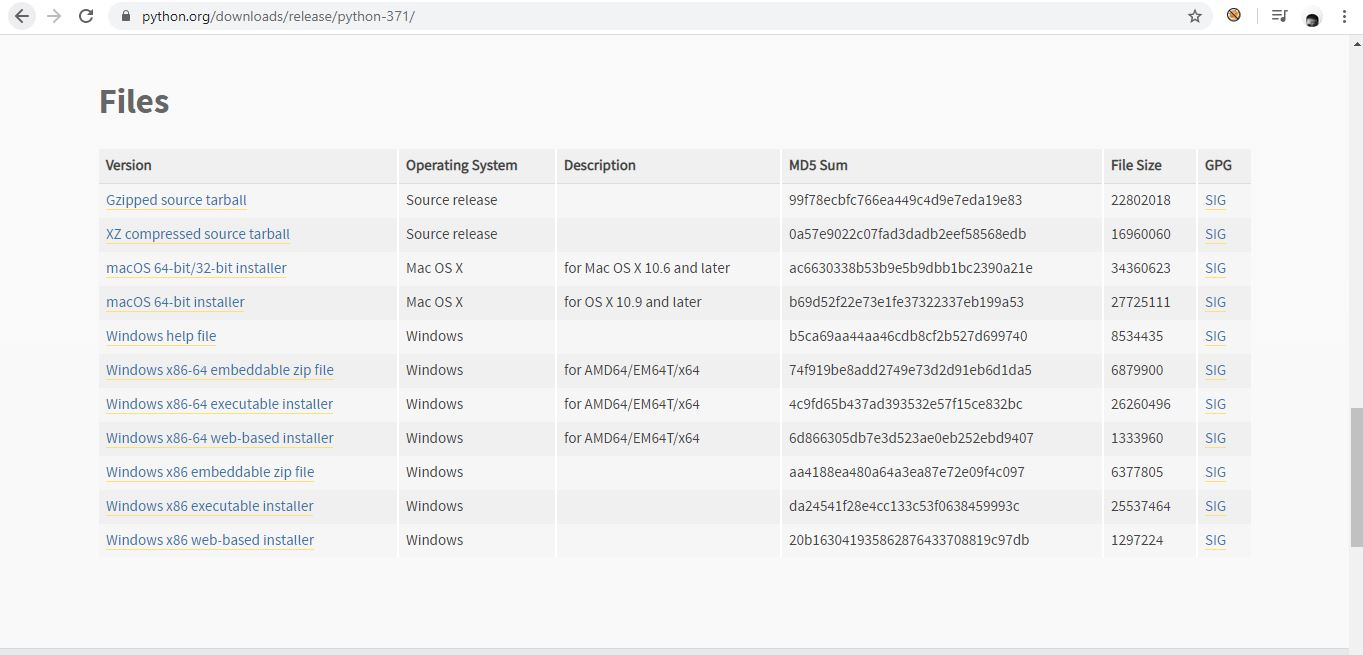
\includegraphics[scale=0.3]{figures/1,10.jpg}
		\caption{Download Python}
		\label{contoh}
		\end{figure}
(lihat PPC Mac OS X 32-bit atau tautan Intel® Mac OS X 64-bit). Menginstal Python dari file .dmg yang diunduh hanya akan menimpa instalasi sistem Python Anda saat ini.

Untuk Mac, ada beberapa pendekatan yang mungkin untuk mendapatkan standar Python 2.7, NumPy, SciPy, dan OpenCV. Semua pendekatan pada akhirnya membutuhkan OpenCV untuk dikompilasi dari sumber menggunakan Alat Pengembang Xcode. Namun, tergantung pada pendekatannya, tugas ini otomatis bagi kami dalam berbagai cara oleh alat pihak ketiga. Kami akan melihat pendekatan semacam ini menggunakan MacPorts atau Homebrew. Alat-alat ini berpotensi melakukan segala yang dapat dilakukan CMake, ditambah lagi membantu kami mengatasi dependensi dan memisahkan pustaka pengembangan kami dari pustaka sistem.
\newpage
\textbf{Tip}

Saya merekomendasikan MacPorts, terutama jika Anda ingin mengkompilasi OpenCV dengan dukungan kamera mendalam melalui OpenNI dan SensorKinect. Tambalan dan skrip yang relevan, termasuk beberapa yang saya kelola, siap pakai untuk MacPorts. Sebaliknya, Homebrew saat ini tidak memberikan solusi yang sudah jadi untuk mengkompilasi OpenCV dengan dukungan kamera yang dalam. Sebelum melanjutkan, pastikan bahwa Alat Pengembang Xcode disiapkan dengan benar:

Unduh dan instal Xcode dari Mac App Store atau \begin{verbatim}https://developer.apple.com/xcode/downloads/ \end{verbatim} Selama instalasi, jika ada opsi untuk menginstal Command Line Tools, pilihlah.

Buka Xcode dan terima perjanjian lisensi.

Langkah terakhir diperlukan jika penginstal tidak memberi kami opsi untuk menginstal Alat Baris Perintah. Arahkan ke Xcode, Preferensi, Unduh, dan klik tombol Instal di sebelah Command Line Tools. Tunggu instalasi untuk menyelesaikan dan keluar dari Xcode.

Atau, Anda dapat menginstal alat baris perintah Xcode dengan menjalankan perintah berikut (di terminal):
\begin{verbatim}
$ xcode-select –install
\end{verbatim}
Sekarang, kami memiliki kompiler yang diperlukan untuk pendekatan apa pun.

Menggunakan MacPorts dengan paket yang sudah jadi

Kita bisa menggunakan manajer paket MacPorts untuk membantu kita mengatur Python 2.7, NumPy, dan OpenCV. MacPorts menyediakan perintah terminal yang mengotomatiskan proses mengunduh, mengkompilasi, dan menginstal berbagai perangkat lunak sumber terbuka (OSS). MacPorts juga menginstal dependensi sesuai kebutuhan. Untuk setiap perangkat lunak, dependensi dan resep bangunan didefinisikan dalam file konfigurasi yang disebut Portfile. Repositori MacPorts adalah kumpulan dari Portfiles.

Mulai dari sistem di mana Xcode dan alat-alat command-line-nya sudah diatur, langkah-langkah berikut akan memberi kita instalasi OpenCV melalui MacPorts:
\newpage
\begin{enumerate}
	\item Unduh dan instal MacPorts dari \begin{verbatim} http://www.macports.org/install.php. \end{verbatim}
		\begin{figure}[ht]
		\centering
		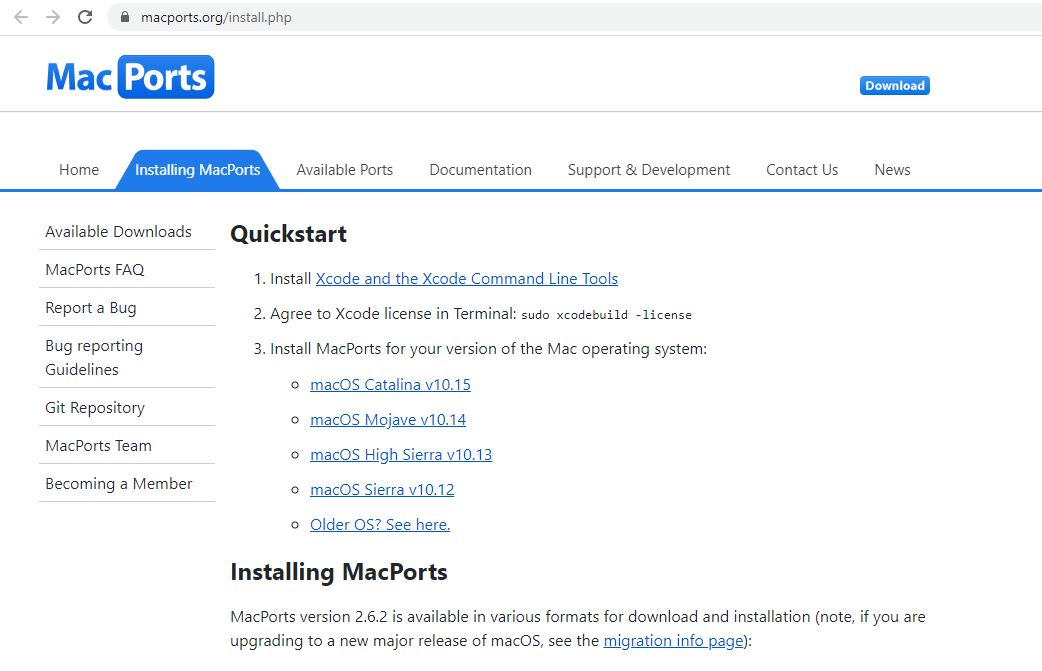
\includegraphics[scale=0.4]{figures/1,11.jpg}
		\caption{Download MacPorts}
		\label{contoh}
		\end{figure}
	\item Jika Anda ingin dukungan untuk kamera kedalaman Kinect, Anda perlu memberi tahu MacPorts tempat untuk mengunduh Portfile khusus yang telah saya tulis. Untuk melakukannya, edit

	/opt/local/etc/macports/sources.conf (dengan asumsi bahwa MacPorts diinstal ke lokasi default). Tepat di atas garis,

	rsync: //rsync.macports.org/release/ports/ [default], tambahkan baris berikut:

	http://nummist.com/opencv/ports.tar.gz

	Simpan file. Sekarang, MacPorts tahu bahwa ia harus mencari Portfile di repositori online saya terlebih dahulu, dan kemudian repositori online default.
	\item Buka terminal dan jalankan perintah berikut untuk memperbarui MacPorts:
	\begin{verbatim}
	$ sudo port selfupdate
	\end{verbatim}
	Saat diminta, masukkan kata sandi Anda.
	\item Sekarang (jika kita menggunakan repositori saya), jalankan perintah berikut untuk menginstal OpenCV dengan binding Python 2.7 dan dukungan untuk kamera kedalaman, termasuk Kinect:
	\begin{verbatim}
	$ sudo port instal opencv + python27 + openni_sensorkinect
	\end{verbatim}
	Atau (dengan atau tanpa repositori saya), jalankan perintah berikut untuk menginstal OpenCV dengan binding Python 2.7 dan dukungan untuk kamera kedalaman, tidak termasuk Kinect:
	\begin{verbatim}
	$ sudo port instal opencv + python27 + openni
	\end{verbatim}

	\textbf{Catatan}

	Ketergantungan, termasuk Python 2.7, NumPy, OpenNI, dan (dalam contoh pertama) SensorKinect, diinstal secara otomatis juga. Dengan menambahkan  python27 ke perintah, kami menentukan bahwa kami ingin varian OpenCV (membangun konfigurasi) dengan Python 2.7 binding. Demikian pula, menambahkan \verb|openni_sensorkinect| menentukan varian dengan dukungan seluas mungkin untuk kamera kedalaman melalui OpenNI dan SensorKinect. Anda dapat menghilangkan \verb|+ openni_sensorkinect| jika Anda tidak bermaksud menggunakan kamera kedalaman, atau Anda dapat menggantinya dengan \verb|+| openni jika Anda bermaksud menggunakan kamera kedalaman yang kompatibel dengan OpenNI tetapi tidak dengan Kinect. Untuk melihat daftar lengkap varian yang tersedia sebelum menginstal, kita dapat memasukkan perintah berikut:
	\begin{verbatim}
	$ port varian opencv
	\end{verbatim}
	Bergantung pada kebutuhan penyesuaian kami, kami dapat menambahkan varian lain ke perintah pemasangan. Untuk fleksibilitas yang lebih besar, kita dapat menulis varian kita sendiri (seperti yang dijelaskan di bagian selanjutnya).
	\item Juga, jalankan perintah berikut untuk menginstal SciPy:
	\begin{verbatim}
	$ sudo port install py27-scipy
	\end{verbatim}
	\item Eksekusi instalasi Python bernama python2.7. Jika kita ingin menautkan python default yang dapat dieksekusi ke python2.7, mari kita juga jalankan perintah ini:
	\begin{verbatim}
	$ sudo port install python_select
	$ sudo port pilih python python27
	\end{verbatim}
\end{enumerate}

\newpage
\textbf{Menggunakan MacPorts dengan paket kustom Anda sendiri}

Dengan beberapa langkah tambahan, kita dapat mengubah cara MacPorts mengkompilasi OpenCV atau perangkat lunak lainnya. Seperti disebutkan sebelumnya, resep build MacPorts didefinisikan dalam file konfigurasi yang disebut Portfiles. Dengan membuat atau mengedit Portfile, kita dapat mengakses alat bantu yang sangat dapat dikonfigurasi, seperti CMake, sementara juga memanfaatkan fitur MacPorts, seperti resolusi ketergantungan.

Mari kita asumsikan bahwa kita sudah menginstal MacPorts. Sekarang, kita dapat mengkonfigurasi MacPorts ke
gunakan Portfile khusus yang kita tulis:

\begin{enumerate}
	\item Buat folder di suatu tempat untuk menampung Portfiles khusus kami. Kami akan merujuk ke folder ini sebagai \begin{verbatim} <local_repository> \end{verbatim}
	\item Edit file /opt/local/etc/macports/sources.conf (dengan anggapan bahwa MacPorts diinstal ke lokasi default). Tepat di atas
	\begin{verbatim} rsync: //rsync.macports.org/release/ports/ default baris, tambahkan baris ini:
	file: // <local_repository>
	Misalnya, jika <local_repository> adalah / Users / Joe / Portfiles, tambahkan baris berikut:
	file: /// Pengguna / Joe / Portfiles \end{verbatim}
	Catat tiga tebasan dan simpan file. Sekarang, MacPorts tahu bahwa ia harus mencari Portfiles di \begin{verbatim} <local_repository> \end{verbatim} terlebih dahulu, dan kemudian, repositori online default-nya.
	\item Buka terminal dan perbarui MacPorts untuk memastikan bahwa kami memiliki Portfile terbaru dari repositori default:
	\begin{verbatim} $ sudo port selfupdate \end{verbatim}
	\item Mari kita salin opencv Portfile repositori default sebagai contoh. Kami juga harus menyalin struktur direktori, yang menentukan bagaimana paket dikategorikan oleh MacPorts:
	\begin{verbatim} $ mkdir <local_repository> / graphics /
	$ cp
	/opt/local/var/macports/sources/rsync.macports.org/release/ports/graphi
	cs / opencv <local_repository> / grafis \end{verbatim}
\newpage
	Sebagai alternatif, untuk contoh yang menyertakan dukungan Kinect, kita dapat mengunduh repositori online saya dari \verb|http://nummist.com/opencv/ports.tar.gz|
		\begin{figure}[ht]
		\centering
		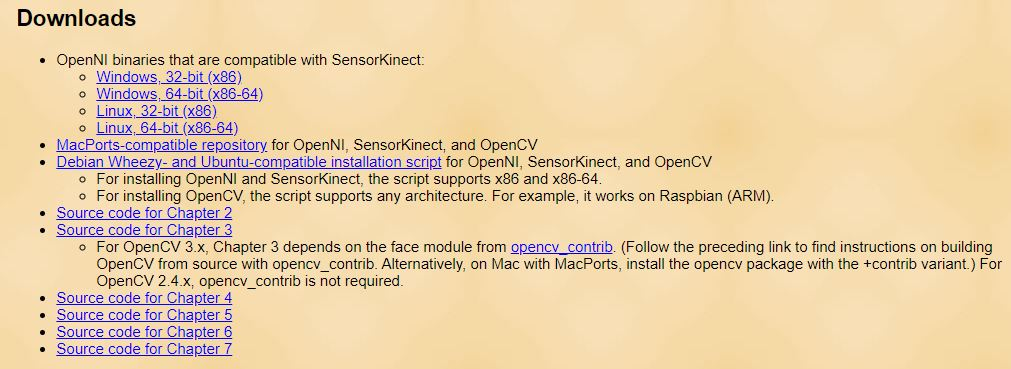
\includegraphics[scale=0.3]{figures/1,12.jpg}
		\caption{Download Kinect}
		\label{contoh}
		\end{figure}
	, unzip, dan salin seluruh folder grafiknya ke \begin{verbatim} <local_repository> \end{verbatim}:
	\begin{verbatim} $ cp <unzip_destination> / graphics <local_repository> \end{verbatim}
	\item Edit \begin{verbatim} <local_repository>/graphics/opencv/Portfile. \end{verbatim} Perhatikan bahwa file ini menentukan flag konfigurasi, dependensi, dan varian CMake. Untuk detail tentang pengeditan Portfile, buka \begin{verbatim} http://guide.macports.org/#development. \end{verbatim}
		\begin{figure}[ht]
		\centering
		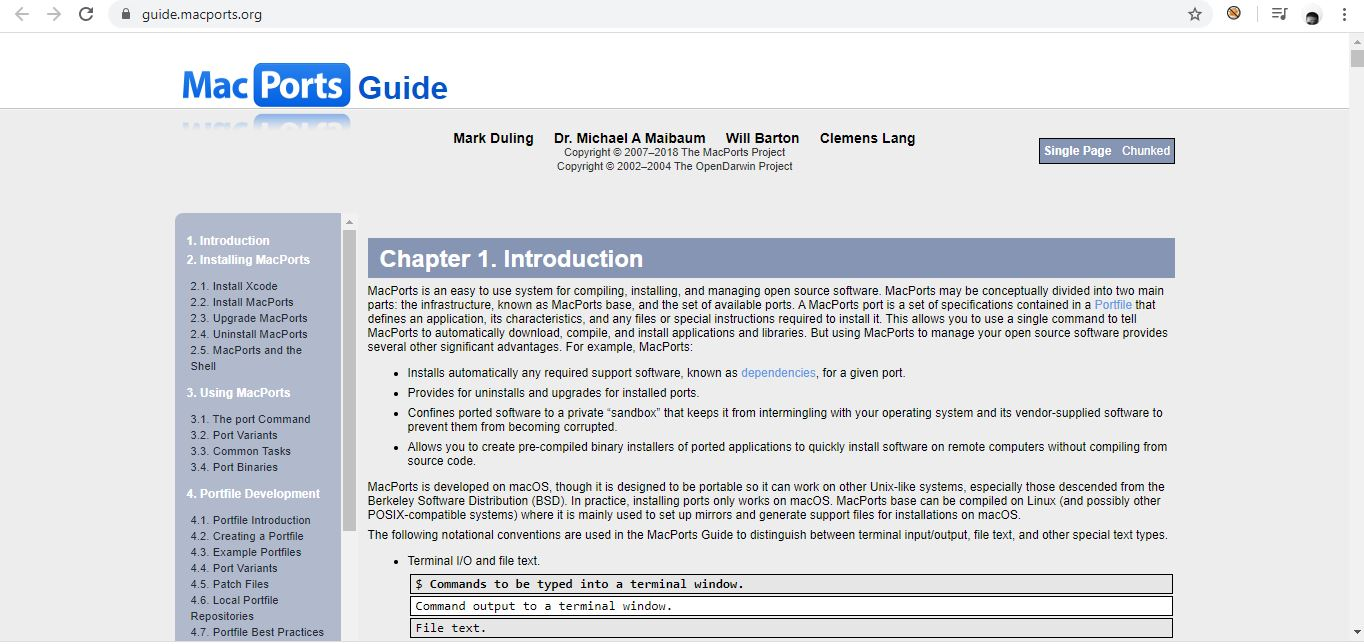
\includegraphics[scale=0.4]{figures/1,13.jpg}
		\caption{Tutorial pada website tersebut}
		\label{contoh}
		\end{figure}
\newpage
	Untuk melihat flag konfigurasi CMake mana yang relevan dengan OpenCV, kita perlu melihat kode sumbernya. Unduh arsip kode sumber dari
	\verb|https://github.com/Itseez/opencv/archive/3.0.0.zip| unzip ke lokasi mana pun, dan baca \verb|<unzip_destination> /OpenCV-3.0.0/CMakeLists.txt.|
	Setelah melakukan pengeditan ke Portfile, simpanlah.
	\item Sekarang, kita perlu membuat file indeks di repositori lokal kita sehingga MacPorts dapat menemukan Portfile baru:
	\begin{verbatim} $ cd <local_repository>
	$ portindex \end{verbatim}
	\item Mulai sekarang, kita dapat memperlakukan file pembuka kustom kita sama seperti paket MacPorts lainnya. Sebagai contoh, kita dapat menginstalnya sebagai berikut:
	\begin{verbatim} $ sudo port instal opencv + python27 + openni_sensorkinect \end{verbatim}
	Perhatikan bahwa Portfile repositori lokal kami lebih diutamakan daripada Portfile repositori default karena urutan urutannya.
	/opt/local/etc/macports/sources.conf.
\end{enumerate}

\newpage
\textbf{Menggunakan Homebrew dengan paket yang sudah jadi (tidak ada dukungan untuk kamera kedalaman)}

Homebrew adalah manajer paket lain yang dapat membantu kami. Biasanya, MacPorts dan Homebrew tidak boleh diinstal pada mesin yang sama. 

Mulai dari sistem di mana Xcode dan alat-alat command-line-nya sudah diatur, langkah-langkah berikut akan memberi kita instalasi OpenCV melalui Homebrew:

\begin{enumerate}
	\item Buka terminal dan jalankan perintah berikut untuk menginstal Homebrew:
	\begin{verbatim}$ ruby ​​-e "$ (curl -fsSkLraw.github.com/mxcl/homebrew/go)" \end{verbatim} 
	\item Tidak seperti MacPorts, Homebrew tidak secara otomatis menempatkan executable-nya di PATH. Untuk melakukannya, buat atau edit file \begin{verbatim} ~/.profile \end{verbatim} dan tambahkan baris ini di bagian atas kode:
	\begin{verbatim} 
	eksport PATH = / usr / local / bin: / usr / local / sbin: $ PATH
	\end{verbatim}
	Simpan file dan jalankan perintah ini untuk menyegarkan PATH:
	\begin{verbatim} 
	$ source ~/.profile
	\end{verbatim}
	Perhatikan bahwa executable yang diinstal oleh Homebrew sekarang diutamakan daripada executable yang diinstal oleh sistem.

	\item Untuk laporan diagnostik mandiri Homebrew, jalankan perintah berikut:
	\begin{verbatim} 
	$ brew doctor
	\end{verbatim}
	Ikuti saran pemecahan masalah yang diberikannya.
	\item Sekarang, perbarui Homebrew:
	\begin{verbatim} 
	$ brew update
	\end{verbatim}
	\item Jalankan perintah berikut untuk menginstal Python 2.7:
	\begin{verbatim} 
	$ brew install python
	\end{verbatim}	
	\item Sekarang, kita dapat menginstal NumPy. Pilihan paket pustaka Python Homebrew terbatas, jadi kami menggunakan alat manajemen paket terpisah yang disebut pip, yang dilengkapi dengan Homebrew Python:
	\begin{verbatim} 
	$ pip install numpy
	\end{verbatim}
	\item SciPy berisi beberapa kode Fortran, jadi kita memerlukan kompiler yang sesuai. Kita dapat menggunakan Homebrew untuk menginstal kompiler gfortran:
	\begin{verbatim} 
	$ brew install gfortran
	\end{verbatim}
	Sekarang, kita dapat menginstal SciPy:
	\begin{verbatim} 
	$ pip install scipy
	\end{verbatim}
	\item Untuk menginstal OpenCV pada sistem 64-bit (semua perangkat keras Mac baru sejak akhir 2006), jalankan
	perintah berikut:
	
\begin{enumerate}

\newpage
\textbf{Tip}
\newline
\textbf{Mengunduh kode contoh}
\newline

Anda dapat mengunduh file kode contoh untuk semua buku Penerbitan Packt yang telah Anda beli dari akun Anda di \begin{verbatim} http://www.packtpub.com.\end{verbatim} Jika Anda membeli buku ini di tempat lain, Anda dapat mengunjungi \begin{verbatim} http://www.packtpub.com/support\end{verbatim} dan mendaftar agar file-file tersebut diemail langsung kepada Anda.
		\begin{figure}[ht]
		\centering
		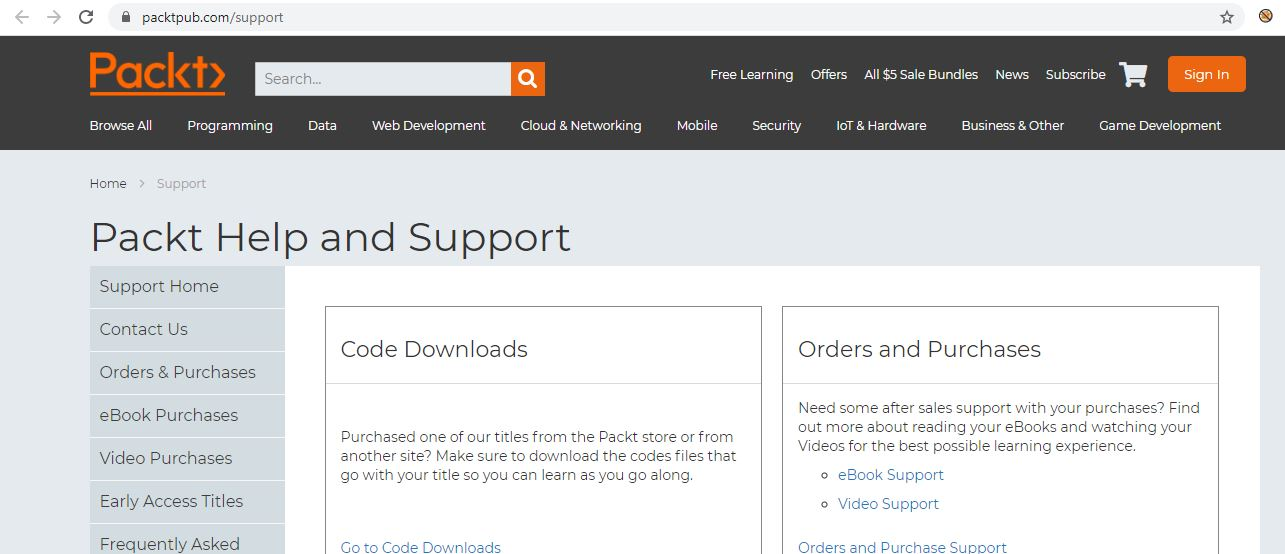
\includegraphics[scale=0.4]{figures/1,14.jpg}
		\caption{Website packtpub}
		\label{contoh}
		\end{figure}

\textbf{Menggunakan Homebrew dengan paket kustom Anda sendiri}
\newline
Homebrew memudahkan untuk mengedit definisi paket yang ada:
\begin{verbatim} 
$ brew edit opencv
\end{verbatim}

Definisi paket sebenarnya adalah skrip dalam bahasa pemrograman Ruby. Kiat untuk mengeditnya dapat ditemukan di halaman Wiki Homebrew di \begin{verbatim} https://github.com/mxcl/homebrew/wiki/Formula-Cookbook. \end{verbatim} Sebuah skrip dapat menentukan flag konfigurasi Make atau CMake, antara lain.

Untuk melihat flag konfigurasi CMake mana yang relevan dengan OpenCV, kita perlu melihat kode sumbernya. Unduh arsip kode sumber dari \begin{verbatim} https://github.com/Itseez/opencv/archive/3.0.0.zip \end{verbatim}, unzip ke lokasi mana pun, dan baca \begin{verbatim} <unzip_destination>/OpenCV-2.4.3/CMakeLists.txt. \end{verbatim}
Setelah mengedit skrip Ruby, simpan.
Paket khusus dapat diperlakukan seperti biasa. Misalnya, dapat diinstal sebagai berikut:
\begin{verbatim} 
$ brew install opencv
\end{verbatim}


\newpage
\subsection {Instalasi pada Ubuntu}

Pertama dan terpenting, berikut adalah catatan singkat tentang versi Ubuntu dari sistem operasi: Ubuntu memiliki siklus rilis 6 bulan di mana setiap rilis adalah versi minor .04 atau .10 dari versi utama (14 pada saat penulisan). Namun, setiap dua tahun, Ubuntu merilis versi yang diklasifikasikan sebagai dukungan jangka panjang (LTS) yang akan memberi Anda dukungan lima tahun oleh Canonical (perusahaan di belakang Ubuntu). Jika Anda bekerja di lingkungan perusahaan, disarankan untuk menginstal salah satu versi LTS. Yang terbaru yang tersedia adalah 14,04.


Ubuntu hadir dengan Python 2.7 yang sudah diinstal. Repositori Ubuntu standar berisi paket OpenCV 2.4.9 tanpa dukungan untuk kamera yang dalam. Pada saat penulisan ini, OpenCV 3 belum tersedia melalui repositori Ubuntu, jadi kita harus membuatnya dari sumber. Untungnya, sebagian besar sistem Unix-like dan Linux datang dengan semua perangkat lunak yang diperlukan untuk membangun proyek dari awal yang sudah diinstal. Ketika dibangun dari sumber, OpenCV dapat mendukung kamera kedalaman melalui OpenNI dan SensorKinect, yang tersedia sebagai binari yang dikompilasi dengan skrip instalasi.

\par
\textbf {Menggunakan repositori Ubuntu (tidak ada dukungan untuk kamera kedalaman)}

Kita dapat menginstal Python dan semua dependensi yang diperlukan menggunakan manajer paket apt, dengan menjalankan perintah berikut:
\begin{verbatim}
> sudo apt-get install build-essential
> sudo apt-get install cmake git libgtk2.0-dev pkg-config libavcodecdev
libavformat-dev libswscale-dev
> sudo apt-get install python-dev python-numpy libtbb2 libtbb-dev libjpegdev libpng-dev libtiff-dev libjasper-dev libdc1394-22-dev 
\end{verbatim}
Secara setara, kita bisa menggunakan Ubuntu Software Center, yang merupakan tampilan grafis apt package manager.

\newpage
\textbf {Membangun OpenCV dari sumber}
Sekarang kita telah menginstal seluruh tumpukan Python dan cmake, kita dapat membangun OpenCV.
Pertama, kita perlu mengunduh kode sumbernya
\verb| https: //github.com/Itseez/opencv/archive/3.0.0-beta.zip. |
Ekstrak arsip dan pindahkan ke folder yang tidak di-zip di terminal.
Kemudian, jalankan perintah berikut:
\begin{verbatim}
> mkdir build
> cd build
> cmake -D CMAKE_BUILD_TYPE =Release -D CMAKE_INSTALL_PREFIX =/usr/local ..
> make
> make install 
\end{verbatim}

Setelah instalasi berakhir, Anda mungkin ingin melihat contoh Python OpenCV di
\verb|<opencv_folder>/opencv/samples/python| dan
\verb|<script_folder>/opencv/samples/python2.|

Instalasi pada sistem mirip Unix lainnya
Pendekatan untuk Ubuntu (seperti yang dijelaskan sebelumnya) kemungkinan akan bekerja pada distribusi Linux apa pun yang berasal dari Ubuntu 14.04 LTS atau Ubuntu 14.10 sebagai berikut:
Kubuntu 14.04 LTS atau Kubuntu 14.10
Xubuntu 14.04 LTS atau Xubuntu 14.10
Linux Mint 17

Pada Debian Linux dan turunannya, manajer paket apt berfungsi sama seperti di Ubuntu, meskipun paket yang tersedia mungkin berbeda.

Di Gentoo Linux dan turunannya, manajer paket Portage mirip dengan MacPorts (seperti dijelaskan sebelumnya), meskipun paket yang tersedia mungkin berbeda.

Pada turunan FreeBSD, proses instalasi sekali lagi mirip dengan MacPorts; sebenarnya, MacPorts berasal dari sistem instalasi port yang diadopsi pada FreeBSD. Bacalah Buku Pegangan FreeBSD yang luar biasa di \newline \verb|https://www.freebsd.org/doc/handbook/| untuk ikhtisar proses instalasi perangkat lunak.
		\begin{figure}[ht]
		\centering
		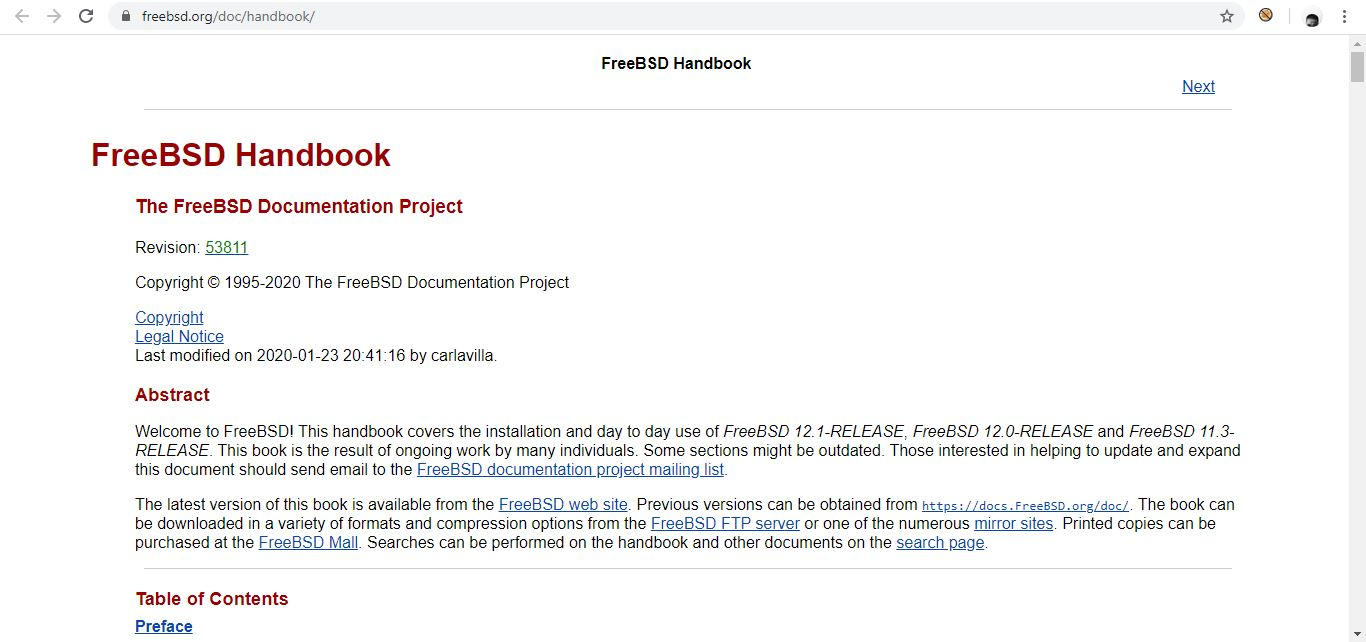
\includegraphics[scale=0.4]{figures/1,15.jpg}
		\caption{FreeBSD}
		\label{contoh}
		\end{figure}
\newpage
Pada sistem mirip Unix lainnya, manajer paket dan paket yang tersedia mungkin berbeda. Konsultasikan dokumentasi manajer paket Anda dan cari paket dengan opencv di namanya. Ingatlah bahwa OpenCV dan binding Python-nya dapat dipecah menjadi beberapa
paket.

Juga, cari semua catatan instalasi yang diterbitkan oleh penyedia sistem, pengelola repositori, atau komunitas. Karena OpenCV menggunakan driver kamera dan codec media, membuat semua fungsinya berfungsi dapat menjadi rumit pada sistem dengan dukungan multimedia yang buruk. Dalam beberapa keadaan, paket sistem mungkin perlu dikonfigurasi ulang atau diinstal ulang untuk kompatibilitas.

Jika paket tersedia untuk OpenCV, periksa nomor versinya. OpenCV 3 atau lebih tinggi direkomendasikan untuk tujuan buku ini. Juga, periksa apakah paket menawarkan binding Python dan dukungan kamera mendalam melalui OpenNI dan SensorKinect. Terakhir, periksa apakah ada orang di komunitas pengembang yang melaporkan keberhasilan atau kegagalan dalam menggunakan paket.

Jika, sebaliknya, kami ingin melakukan pembuatan kustom OpenCV dari sumber, mungkin bermanfaat untuk merujuk ke skrip instalasi untuk Ubuntu (seperti yang dibahas sebelumnya) dan menyesuaikannya dengan manajer paket dan paket yang ada di sistem lain.


\newpage
\subsection {Instalasi modul Contrib}
Berbeda dengan OpenCV 2.4, beberapa modul terdapat dalam repositori yang disebut \verb|opencv_contrib|, yang tersedia di \verb|https://github.com/Itseez/opencv_contrib.| Saya sangat merekomendasikan menginstal modul ini karena mengandung fungsionalitas tambahan yang tidak termasuk dalam OpenCV, seperti modul pengenalan wajah.
Setelah diunduh (baik melalui zip atau git, saya sarankan git agar Anda dapat tetap up to date dengan perintah git pull sederhana), Anda dapat menjalankan kembali perintah cmake Anda untuk memasukkan pembangunan OpenCV dengan modul \verb|opencv_contrib| sebagai berikut:
\begin{verbatim}
cmake -DOPENCV_EXTRA_MODULES_PATH = <opencv_contrib> / modules
<opencv_source_directory>
\end{verbatim}

Jadi, jika Anda telah mengikuti prosedur standar dan membuat direktori build di folder unduhan OpenCV Anda, Anda harus menjalankan perintah berikut:

\begin{verbatim}
mkdir build && cd build
cmake -D CMAKE_BUILD_TYPE = Lepaskan -DOPENCV_EXTRA_MODULES_PATH =
<opencv_contrib> / modules -D CMAKE_INSTALL_PREFIX = / usr / local ..
make
\end{verbatim}

\newpage
\subsection {PyCharm}
Pycharm merupakan tools untuk menjalankan program python didalamnya sudah terdapat berbagai macam library dari python itu sendiri, kita hanya perlu mencari library yang kita butuhkan kemudian klik install, maka kita tidak perlu melakukan hal hal yang telah di contohkan untuk menginstall opencv pada windows atau yang lainnya. Yang perlu kita lakukan yang pertama kalinya adalah kita mendownload aplikasi PyCharm. \newline \verb|https://www.jetbrains.com/pycharm/download/#section=windows| \newline 
		\begin{figure}[ht]
		\centering
		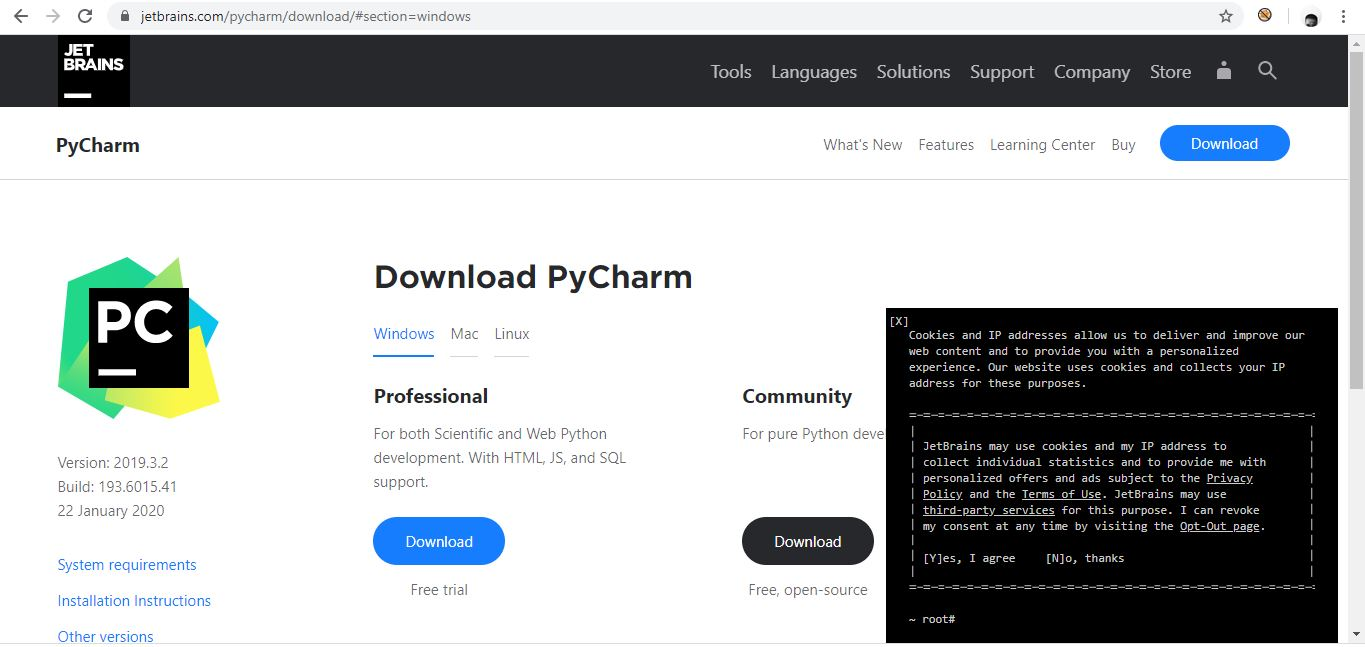
\includegraphics[scale=0.4]{figures/1,16.jpg}
		\caption{Pycharm}
		\label{contoh}
		\end{figure}
\newpage
Kemudian lakukan installasi, setelah istallasi selesai selanjutnya kita buka aplikasi kemudian pilih file kemudian settings.
		\begin{figure}[ht]
		\centering
		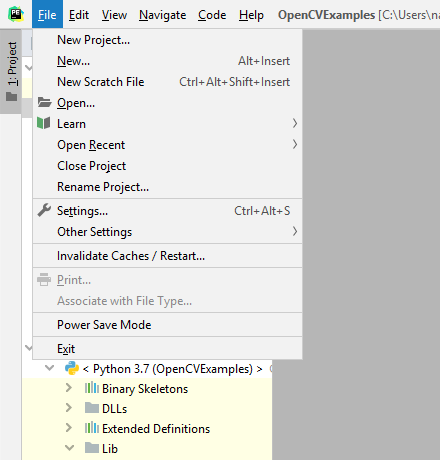
\includegraphics[scale=0.4]{figures/1,17.png}
		\caption{Pycharm Settings}
		\label{contoh}
		\end{figure}
\newline
Kemudian pilih project interpreter, lalu klik tambah pada pojok kanan, maka tampilannya akan seperti ini:
		\begin{figure}[ht]
		\centering
		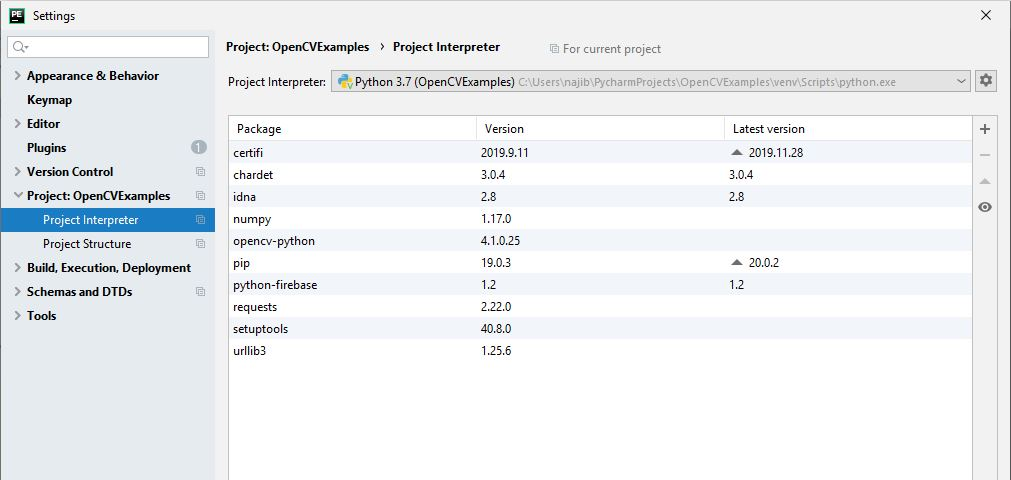
\includegraphics[scale=0.4]{figures/1,18.jpg}
		\caption{Install library}
		\label{contoh}
		\end{figure}
\newpage
Setelah masuk pada tampilan ini kita cari library apa yang kita butuhkan untuk menjalankan project yang akan kita bangun, karna bahasan kita pada saat ini yaitu OPENCV maka yang kita cari adalah OpenCV, Setelah menemukannya kita langsung saja klik install kira kira membutuhkan waktu lumayan lama, jika internet kita stabil kurang lebih 20-30 menit waktu yang di butuhkan untuk menginstall opencv ini.
		\begin{figure}[ht]
		\centering
		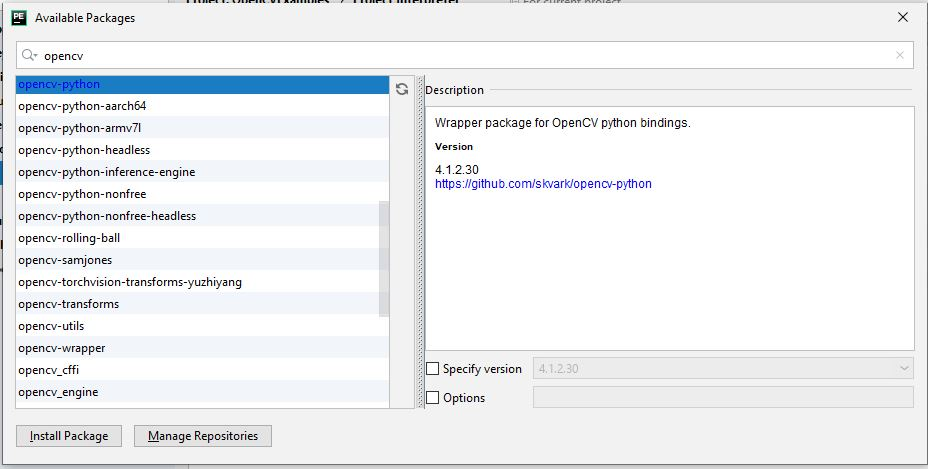
\includegraphics[scale=0.4]{figures/1,19.jpg}
		\caption{Install OpenCV}
		\label{contoh}
		\end{figure}